%%%%%%%%%%%%%%%%%%%%%%%%%%%%%%%%%%%%%%%%%%%%%%%%%%%%%
%% File: main.tex
%% Author: Evangelos Stamos (estamos@e-ce.uth.gr)
%% Last update: January, 2020
%% Description: Provides an example of a Diploma Thesis 
%% using the ntua-thesis pdfLaTeX class.
%%
%% Character encoding: UTF-8
%%%%%%%%%%%%%%%%%%%%%%%%%%%%%%%%%%%%%%%%%%%%%%%%%%%%%
%
%
%%%%%%
% 1. use the "modern" or "classic" option to switch between 
% a modern or classic font, respectively.
%
% 2. add/remove the "hyperref" option to enable/disable hyperlinks:
% (remember to remove auxiliary files after adding/removing 
% the "hyperref" option).
%
% 3. add/remove the "printer" option to typeset a printer-friendly 
% (grayscale)/color version of the thesis.
%
% 4. use the "watermark" option to indicate that this is not an actual
% thesis.
%
% 5. use the "histinit" option to enable "historiated initials".
% (If used, all chapter initials declared by the \InitialCharacter{}
% macro are enlarged. If omitted, arguments of \InitialCharacter{}
% are typeset as normal text.)
%
% 6. use the "plain" option to disable tikz graphics in title page
% and part/chapter headers (might help to avoid compilation timeouts).
% Note that "plain" disables CD label and CD cover creation.
%
% 7. use the "noindex" option to (hopefully) avoid compilation timeouts
% when compiling online (disables index generation - note that "\indexGR",
% "\indexEN" invocations need not be removed when toggling this option).
%
% 8. activate the "newlogo" option to use the new official Logo.
%
%%%%%%%%%%%%%%%%%%%%%%%%%%%%%%%%%%%%%%%%%%%%%%%%%%%%%%%%%%%%%%%%%%%%%%%%%%%%%%%
%
\documentclass[modern,hyperref,watermark,histinit,noindex,plain,newlogo]{ntua-thesis}
%
%%%%%%%%%%%%%%%%%%%%%%%%%%%%%%%%%%%%%%%%%%%%%%%%%%%%%%%%%%%%%%%%%%%%%%%%%%%%%%%
%
%
%%%%%%%%%%%%%%%%%%%%%%%%%%%%%%%%%%%%%%%%%%%%%%%%%%%%
%% THESIS INFO 
%%%%%%%%%%%%%%%%%%%%%%%%%%%%%%%%%%%%%%%%%%%%%%%%%%%%
%
% ΤΙΤΛΟΣ ΔΙΠΛΩΜΑΤΙΚΗΣ ΕΡΓΑΣΙΑΣ 
%
% Για εξαναγκασμένες αλλαγές γραμμής χρησιμοποιήστε "\\".
% Αν οι αλλαγές γραμμής πρέπει να είναι διαφορετικές στο εξώφυλλο σε σχέση 
% με το εσώφυλλο (σελ. 3), επαναλάβετε τον τίτλο του εξωφύλλου με τις 
% επιθυμητές αλλαγές γραμμής ως προαιρετικό όρισμα της εντολής \title.
%
% Παραδείγματα:
% 1. Όμοιος τίτλος σε εξώφυλλο και εσώφυλλο, με αυτόματες αλλαγές γραμμής:
%	    \title{Πρότυπο Σύστημα Ομότιμων Κόμβων Βασισμένο σε Σχήματα \en{RDF}}
% 2. Όμοιος τίτλος σε εξώφυλλο και εσώφυλλο, με αλλαγή γραμμής μετά τη λέξη
% "Σύστημα":
%	    \title{Πρότυπο Σύστημα \\ Ομότιμων Κόμβων Βασισμένο σε Σχήματα \en{RDF}}
% 3. Διαφορετικές αλλαγές γραμμής σε εξώφυλλο και εσώφυλλο. Στο εξώφυλλο 
% έχουμε αλλαγή γραμμής μετά τη λέξη "Σύστημα", ενώ στο εσώφυλλο η αλλαγή
% γραμμής ακολουθεί τη λέξη "Ομότιμων":
%	    \title[Πρότυπο Σύστημα \\ Ομότιμων Κόμβων Βασισμένο %
%           σε Σχήματα \en{RDF}]% (προαιρετικό όρισμα)
%           {Πρότυπο Σύστημα Ομότιμων \\ Κόμβων Βασισμένο σε %
%           Σχήματα \en{RDF}}% (υποχρεωτικό όρισμα)
%
	\title{Πρότυπο Σύστημα Ομότιμων Κόμβων \\Βασισμένο σε Σχήματα \en{RDF}}
%%
%
%% -------------------------------------------------------------------
%% ΥΠΟΤΙΤΛΟΣ ΔΙΠΛΩΜΑΤΙΚΗΣ ΕΡΓΑΣΙΑΣ (προαιρετικός)
%
% Αν δεν υπάρχει υπότιτλος, τοποθετήστε τον χαρακτήρα του σχολίου "%"
% πριν από την εντολή \subtitle, ή αφήστε κενό το όρισμα της εντολής.
%
% Παράδειγμα:
%%	\subtitle{Μελέτη και υλοποίηση}
	\subtitle{Μελέτη και υλοποίηση}
%
%% -------------------------------------------------------------------
%% ΤΟΥ/ΤΗΣ/ΤΩΝ
%
% "του" ή "της" ή "των", ανάλογα με το φύλο/αριθμό του σπουδαστή ή 
% των σπουδαστών
% Παράδειγμα:
%	\toutis{του}
	\toutis{του}
%
%% -------------------------------------------------------------------
%% ΟΝΟΜΑΤΕΠΩΝΥΜΟ ΣΠΟΥΔΑΣΤΗ ΣΤΑ ΕΛΛΗΝΙΚΑ (ΚΕΦΑΛΑΙΑ, ΓΕΝΙΚΗ ΠΤΩΣΗ)
%
% Για περισσότερους του ενός σπουδαστές, διαχωρίστε με ",".
% Παράδειγμα:
%	\authorNameCapitalGR{ΚΩΝΣΤΑΝΤΙΝΟΥ Δ. ΔΗΜΗΤΡΙΟΥ, ΓΕΩΡΓΙΟΥ Π. ΠΑΝΑΓΑΚΗ}
	\authorNameCapitalGR{ΣΤΑΜΟΥ Φ. ΕΥΑΓΓΕΛΟΥ}
%
%% -------------------------------------------------------------------
%% ΟΝΟΜΑΤΕΠΩΝΥΜΟ ΣΠΟΥΔΑΣΤΗ ΣΤΗ ΛΑΤΙΝΙΚΗ ΜΟΡΦΗ (ΠΕΖΑ)
%
% Δηλώστε εδώ τυχόν ονοματεπώνυμα στη λατινική μορφή, αλλιώς αφήστε
% κενό το όρισμα.
% Για περισσότερους του ενός σπουδαστές, διαχωρίστε με ",".
% Παράδειγμα:
%	\authorNameEN{Albert Einstein, George W. Bush} 
	%\authorNameEN{Albert Einstein} 
%
%% -------------------------------------------------------------------
%% ΟΝΟΜΑΤΕΠΩΝΥΜΟ ΣΠΟΥΔΑΣΤΗ ΣΤΑ ΕΛΛΗΝΙΚΑ (ΠΕΖΑ, ΟΝΟΜΑΣΤΙΚΗ ΠΤΩΣΗ)
%
% Για περισσότερους του ενός σπουδαστές, διαχωρίστε με ",".
% Αν τα ονοματεπώνυμα όλων των σπουδαστών είναι σε λατινική μορφή,
% αφήστε κενό το όρισμα.
% Παράδειγμα:
%	\authorNameGR{Κωνσταντίνος Δημητρίου, Γεώργιος Παναγάκης}
	\authorNameGR{Ευάγγελος Στάμος}
%
%% -------------------------------------------------------------------
%% ΟΝΟΜΑΤΕΠΩΝΥΜΟ ΕΠΙΒΛΕΠΟΝΤΑ ΚΑΘΗΓΗΤΗ
% 
	\supervisor{Ιωάννης Παπαδόπουλος}
%
%% -------------------------------------------------------------------
%% ΤΙΤΛΟΣ ΕΠΙΒΛΕΠΟΝΤΑ ΚΑΘΗΓΗΤΗ
%
	\supervisorTitle{Αναπληρωτής Καθηγητής}
%
%% -------------------------------------------------------------------
%% ΕΠΙΒΛΕΠΩΝ/ΕΠΙΒΛΕΠΟΥΣΑ
%
% "Επιβλέπων" ή "Επιβλέπουσα", ανάλογα με το φύλο του 
% Επιβλέποντα Καθηγητή
	\supervisorMaleFemale{Επιβλέπων}
%
%% -------------------------------------------------------------------
%% ΤΟΠΟΣ/ΜΗΝΑΣ/ΕΤΟΣ ΕΚΔΟΣΗΣ
%
	\thesisPlaceDate{Αθήνα, Νοέμβριος 2020}
%
%% -------------------------------------------------------------------
%% ΤΟΠΟΣ/ΜΗΝΑΣ/ΕΤΟΣ ΣΥΓΓΡΑΦΗΣ (Εμφανίζεται στη σελίδα των ευχαριστιών,
%% αν υπάρχει).
%
	\ackPlaceDate{Αθήνα, Μάιος 2020}
%
%% -------------------------------------------------------------------
%% ΗΜΕΡΟΜΗΝΙΑ ΕΞΕΤΑΣΗΣ
%
	\examinationDate{22α Νοεμβρίου 2020}
%% -------------------------------------------------------------------
%% ΗΜΕΡΟΜΗΝΙΑ ΔΗΛΩΣΗΣ ΠΕΡΙ ΜΗ ΛΟΓΟΚΛΟΠΗΣ
%
	\declarationDate{22 Σεπτεμβρίου 2020}
%
%% -------------------------------------------------------------------
%% ΕΤΟΣ COPYRIGHT
%
	\copyrightYear{2020}
%
%% -------------------------------------------------------------------
%% ΟΝΟΜΑΤΕΠΩΝΥΜΟ 1ου ΕΞΕΤΑΣΤΗ
%
	\firstExaminer{Γρηγόρης Καραγιώργος}
%
%% -------------------------------------------------------------------
%% ΤΙΤΛΟΣ 1ου ΕΞΕΤΑΣΤΗ
%
	\firstExaminerTitle{Επίκουρος Καθηγητής}
%
%% -------------------------------------------------------------------
%% ΟΝΟΜΑΤΕΠΩΝΥΜΟ 2ου ΕΞΕΤΑΣΤΗ
%
	\secondExaminer{Γεώργιος Γεωργίου}
%
%% -------------------------------------------------------------------
%% ΤΙΤΛΟΣ 2ου ΕΞΕΤΑΣΤΗ
%
	\secondExaminerTitle{Επιστ. Συνεργάτης}
%%
%%
%%%%%%%%%%%%%%%%%%%%%%%%%%%%%%%%%%%%%%%%%%%%%%%%%%%%%%%%%%%%%%%%%%%%%%
%% THESIS COLORS: 
%%%%%%%%%%%%%%%%%%%%%%%%%%%%%%%%%%%%%%%%%%%%%%%%%%%%%%%%%%%%%%%%%%%%%%
%%
%% Χρώμα εξωφύλλου - κεφαλαίων
	\chaptercolor{gray!50!brown}
%%
%% Χρώμα παραρτημάτων
	\appendixcolor{brown!60!orange}
%%
%% Χρώμα υπερσυνδέσμων (αν έχει ενεργοποιηθεί η επιλογή "hyperref")
    \hyperlinkcolor{blue}
%%
%% Χρώμα τίτλου εργασίας στο εξώφυλλο (αν δεν έχει ενεργοποιηθεί 
%% η επιλογή "plain")
    \titlecolor{white}
%%
%% Χρώμα υποβάθρου (φόντου) τίτλου εργασίας στο εξώφυλλο (αν δεν έχει 
%% ενεργοποιηθεί η επιλογή "plain")
    \titlebackgroundcolor{gray!60!brown}  
%%
%%
%%%%%%%%%%%%%%%%%%%%%%%%%%%%%%%%%%%%%%%%%%%%%%%%%%%%%%%%%%%%%%%%%%%%%%
%% COVER PAGE IMAGE: 
%%%%%%%%%%%%%%%%%%%%%%%%%%%%%%%%%%%%%%%%%%%%%%%%%%%%%%%%%%%%%%%%%%%%%%
%%
%% Εικόνα εξωφύλλου (προαιρετική)
%% Στην περίπτωση κατά την οποία δεν είναι επιθυμητή η εισαγωγή εικόνας στο εξώφυλλο,
%% διαγράψτε την εντολή \coverpageimage, ή μετατρέψτε την σε σχόλιο (με "%")
%%
%% Σύνταξη:
%%          \coverpageimage{συντελεστής μεγέθυνσης}{όνομα αρχείου εικόνας [πλήρης διαδρομή]}
%%      ή
%%          \coverpageimage[tikz]{συντελεστής μεγέθυνσης}{εντολές TikZ}
%%          (στις εντολές μπορούν να περιλαμβάνονται και δηλώσεις \usetikzlibrary, κ.λπ.)
%%      
%% Παραδείγματα:
%%      - Χρήση εικόνας από το αρχείο "figures/rdf.png" με συντελεστή μεγέθυνσης 0.8:
%%          \coverpageimage{0.8}{figures/rdf.png}
%%      - Χρήση εικόνας TikZ με συντελεστή μεγέθυνσης 0.5:
%%          \coverpageimage[tikz]{0.5}{
%%              \draw[thick, gray] \foreach \x in {18,90,...,306} {
%%                  (\x:4) node{} -- (\x+72:4)
%%                  (\x:4) -- (\x:3) node{}
%%                  (\x:3) -- (\x+15:2) node{}
%%                  (\x:3) -- (\x-15:2) node{}
%%                  (\x+15:2) -- (\x+144-15:2)
%%                  (\x-15:2) -- (\x+144+15:2)
%%              };
%%          }
%%
     \coverpageimage{0.8}{figures/rdf.png}
%%
%%%%%%%%%%%%%%%%%%%%%%%%%%%%%%%%%%%%%%%%%%%%%%%%%%%%%%%%%%%%%%%%%%%%%%
%
% add custom hyphenation rules here
\hyphenation{ο-ποί-α} 
%
%%%%
%
%
%%%%
\begin{document}

\maketitle

\beginfrontmatter
	
% Περίληψη
	\begin{abstract}
Ένα σύστημα ομότιμων κόμβων αποτελείται από ένα σύνολο αυτόνομων
υπολογιστικών κόμβων στο Διαδίκτυο, οι οποίοι συνεργάζονται με
σκοπό την ανταλλαγή δεδομένων. Στα συστήματα ομότιμων κόμβων που
χρησιμοποιούνται ευρέως σήμερα, η αναζήτηση πληροφορίας γίνεται με
χρήση λέξεων κλειδιών. Η ανάγκη για πιο εκφραστικές λειτουργίες,
σε συνδυασμό με την ανάπτυξη του Σημασιολογικού Ιστού, οδήγησε στα
συστήματα ομότιμων κόμβων βασισμένα σε σχήματα. Στα συστήματα αυτά
κάθε κόμβος χρησιμοποιεί ένα σχήμα με βάση το οποίο οργανώνει τα
τοπικά διαθέσιμα δεδομένα. Για να είναι δυνατή η αναζήτηση
δεδομένων στα συστήματα αυτά υπάρχουν δύο τρόποι. Ο πρώτος είναι
όλοι οι κόμβοι να χρησιμοποιούν το ίδιο σχήμα κάτι το οποίο δεν
είναι ευέλικτο. Ο δεύτερος τρόπος δίνει την αυτονομία σε κάθε
κόμβο να επιλέγει όποιο σχήμα θέλει και απαιτεί την ύπαρξη κανόνων
αντιστοίχισης μεταξύ των σχημάτων για να μπορούν να αποτιμώνται οι
ερωτήσεις. Αυτός ο τρόπος προσφέρει ευελιξία όμως δεν υποστηρίζει
την αυτόματη δημιουργία και τη δυναμική ανανέωση των κανόνων, που
είναι απαραίτητες για ένα σύστημα ομότιμων κόμβων.

Στόχος της διπλωματικής εργασίας είναι η ανάπτυξη ενός συστήματος
ομότιμων κόμβων βασισμένο σε σχήματα το οποίο (α) θα επιτρέπει μια
σχετική ευελιξία στην χρήση των σχημάτων και (β) θα δίνει την
δυνατότητα μετασχηματισμού ερωτήσεων χωρίς την ανάγκη διατύπωσης
κανόνων αντιστοίχισης μεταξύ σχημάτων, xρησιμοποιώντας κόμβους με
σχήματα \tl{RDF} που αποτελούν υποσύνολα-όψεις ενός βασικού
σχήματος (καθολικό σχήμα).

   \begin{keywords}
   Σύστημα ομότιμων κόμβων, Σύστημα ομότιμων κόμβων βασισμένο σε
   σχήματα, Σημασιολογικός Ιστός, \tl{RDF/S}, \tl{RQL}, \tl{Jxta}
   \end{keywords}
\end{abstract}



\begin{abstracteng}
\tl{A peer-to-peer system is a set of autonomous computing nodes
(the peers) which cooperate in order to exchange data. The peers
in the peer-to-peer systems that are widely used today, rely on
simple keyword selection in order to search for data. The need for
richer facilities in exchanging data, as well as, the evolution of
the Semantic Web, led to the evolution of the schema-based
peer-to-peer systems. In those systems every node uses a schema to
organize the local data. So there are two ways in order for data
search to be feasible. The first but not so flexible way implies
that every node uses the same schema. The second way gives every
node the flexibility to choose a schema according with its needs,
but on the same time requires the existence of mapping rules in
order for queries to be replied. This way though, doesn't offer
automatic creation and dynamic renewal of the mapping rules which
would be essential for peer-to-peer systems.}

\tl{This diploma thesis aims to the development of a schema-based
peer-to-peer system that allows a certain flexibility for schema
selection and on the same time enables query transformation
without the use of mapping rules. The peers use RDF schemas that
are subsets (views) of a big common schema called global schema.}

   \begin{keywordseng}
    \tl{Peer-to-peer, Schema-based peer-to-peer, Semantic Web, RDF/S, RQL, Jxta}
   \end{keywordseng}

\end{abstracteng}
% Αφιέρωση
	\thesisDedication{στους γονείς μου}
% Ευχαριστίες
	%%%%%%%%%%%%%%%%%%%%%%%%%%%%%%%%%%%%%%%%%%%%%%%%%%%%%%%%%%%%%%%%%
%%
%% use the starred version of the "acknowledgements" environment
%% to omit signatures from this section, e.g.:
%% \begin{acknowledgements*} ... \end{acknowledgements*}
%% 
%%%%%%%%%%%%%%%%%%%%%%%%%%%%%%%%%%%%%%%%%%%%%%%%%%%%%%%%%%%%%%%%%
\begin{acknowledgements}
Θα ήθελα καταρχήν να ευχαριστήσω τον καθηγητή κ. .........
για την επίβλεψη αυτής της διπλωματικής εργασίας και για την
ευκαιρία που μου έδωσε να την εκπονήσω στο εργαστήριο Συστημάτων
Βάσεων Γνώσεων και Δεδομένων. Επίσης ευχαριστώ ιδιαίτερα τον Δρ.
............ για την καθοδήγησή του και την εξαιρετική
συνεργασία που είχαμε. Τέλος θα ήθελα να ευχαριστήσω τους γονείς
μου για την καθοδήγηση και την ηθική συμπαράσταση που μου
προσέφεραν όλα αυτά τα χρόνια.
\end{acknowledgements}
% Πίνακας Περιεχομένων
	\tableofcontents
% Κατάλογος Σχημάτων
	\listoffigures
% Κατάλογος Εικόνων
	\listofillustrations
% Κατάλογος Πινάκων
	\listoftables
% Πρόλογος
	\begin{preface}
Στον πρόλογο αναφέρονται θέματα που δεν είναι επιστημονικά ή τεχνικά, όπως το πλαίσιο που διενεργήθηκε η εργασία, ο τόπος διεξαγωγής, το Εργαστήριο στο οποίο εκπονήθηκε κ.λπ. 
\end{preface}
	
\beginmainmatter

%%%%%%%%%%%%%%%%%%%%%%%%%%%%%%%%%%%%%%%%%%%%%%%%%%%%%
%% INCLUDE YOUR CHAPTERS/SECTIONS HERE
%%
% Εισαγωγή
	\chapter{Εισαγωγή} 
\InitialCharacter{Ο} Παγκόσμιος Ιστός αποτελεί χώρο διακίνησης τεράστιου όγκου
πληροφοριών. Ωστόσο, η συντριπτική πλειοψηφία των πληροφοριών του
Ιστού, είναι προσανατολισμένη προς τον άνθρωπο-χρήστη και δεν
είναι κατανοητή από τις εφαρμογές. Για να αξιοποιηθεί λοιπόν η
διαθέσιμη πληροφορία και να γίνει πιο εύκολη η ανταλλαγή και η
επεξεργασία της, ο Παγκόσμιος Ιστός εξελίσσεται στο Σημασιολογικό
Ιστό.

Ο Σημασιολογικός Ιστός, είναι μια εξέλιξη του σημερινού Ιστού,
μέσα στον οποίο δίνεται καλά ορισμένο νόημα στην πληροφορία που
διακινείται, διευκολύνοντας τη συνεργασία μεταξύ υπολογιστή και
ανθρώπου \cite{LiArTs13}. Πιο συγκεκριμένα δίνει τη
δυνατότητα καλύτερης πρόσβασης σε μεγάλο όγκο πηγών πληροφορίας,
καθώς και πιο αποτελεσματικής διακίνησης των πληροφοριών,
χρησιμοποιώντας δεδομένα που τις περιγράφουν και ονομάζονται
$``$μεταδεδομένα$"$. Η καλύτερη γνώση της σημασίας, της χρήσης και
της ποιότητας των πηγών διευκολύνει σημαντικά τη δυνατότητα
πρόσβασης σε πηγές του Ιστού και την αυτόματη επεξεργασία του
περιεχομένου που υπάρχει διαθέσιμο στο Διαδίκτυο βάσει του
νοήματος και όχι μόνο της μορφής της πληροφορίας.

Ένα από τα πιο βασικά θέματα για την ανάπτυξη του Σημασιολογικού
Ιστού είναι το να μπορούν οι υπολογιστές να ανταλλάσσουν δεδομένα
 μεταξύ εφαρμογών. Σε ένα ανοιχτό περιβάλλον όπως
είναι ο Σημασιολογικός Ιστός χρειάζεται ένα ευέλικτο και δυναμικό
μοντέλο ανταλλαγής δεδομένων όπως είναι τα συστήματα ομότιμων
κόμβων \en{(Peer-to-Peer systems)}.

Ένα σύστημα ομότιμων κόμβων αποτελείται από ένα σύνολο αυτόνομων
υπολογιστικών κόμβων, οι οποίοι συνεργάζονται με σκοπό την
ανταλλαγή δεδομένων. Τα συστήματα ομότιμων κόμβων που
χρησιμοποιούνται ευρέως σήμερα κυρίως για την ανταλλαγή αρχείων
μουσικής, έχουν πολύ μικρές δυνατότητες διαχείρισης δεδομένων. Η
αναζήτηση πληροφορίας στα περισσότερα από αυτά γίνεται με χρήση
λέξεων κλειδιών \en{(keyword-based search)}.

Η ανάγκη για πιο εκφραστικές λειτουργίες, σε συνδυασμό με την
ανάπτυξη του Σημασιολογικού Ιστού, οδήγησε στα συστήματα ομότιμων
κόμβων που είναι βασισμένα σε σχήματα \en{(schema-based
peer-to-peer systems)}. Στα συστήματα αυτά κάθε κόμβος
χρησιμοποιεί ένα σχήμα με βάση το οποίο οργανώνει τα τοπικά
διαθέσιμα δεδομένα. Οι τεχνολογίες του Σημασιολογικού Ιστού δίνουν
τη δυνατότητα οργάνωσης των δεδομένων μέσω σχημάτων που τα
περιγράφουν.

Το πλαίσιο \en{RDF} είναι ένα τέτοιο εργαλείο αναπαράστασης
μεταδεδομένων. Σε ένα \en{RDF} αρχείο ορίζονται δηλώσεις για
αντικείμενα του Ιστού όπως σελίδες, συγγραφείς, προγράμματα κ.τ.λ.
Μια επέκταση του πλαισίου \en{RDF} είναι το \en{RDF Schema} το
οποίο παρέχει μηχανισμούς περιγραφής σχετικών αντικειμένων του
Ιστού καθώς και των σχέσεων μεταξύ τους. Το \en{RDF Schema}
βασίζεται σε κλάσεις και ιδιότητες έννοιες γνωστές από το χώρο των
Αντικειμενοστρεφών συστημάτων. Η βασική διαφορά είναι ότι στο
πλαίσιο \en{RDF} οι ιδιότητες ορίζονται ανεξάρτητα από τις
κλάσεις.

Χρησιμοποιώντας λοιπόν τις τεχνολογίες του Σημασιολογικού Ιστού
μπορούμε να δημιουργήσουμε συστήματα ομότιμων κόμβων με αυξημένη
διαλειτουργικότητα τα οποία θα ανταλλάσσουν μεταξύ τους πληροφορία
με νόημα και θα έχουν τη δυνατότητα διατύπωσης ερωτήσεων πιο
εκφραστικών από αυτές που βασίζονται σε λέξεις κλειδιά.


\section{Αντικείμενο της διπλωματικής}
Το βασικό ζήτημα που προκύπτει για τα συστήματα ομότιμων κόμβων
που είναι βασισμένα σε σχήματα, είναι πώς θα μπορούν οι κόμβοι να
αναζητούν και να ανταλλάσσουν δεδομένα, διατηρώντας την αυτονομία
τους. Δύο προσεγγίσεις έχουν προταθεί στην βιβλιογραφία:
\begin{enumerate}
\item Η πρώτη προσέγγιση απαιτεί να υπάρχει ένα κεντρικό σχήμα το
οποίο θα χρησιμοποιούν όλοι οι κόμβοι \cite{LaTeXProject}. Οι
ερωτήσεις διατυπώνονται και αποτιμούνται με βάση το ίδιο σχήμα.
Μια τέτοια λύση θα ήταν καλή για περιβάλλοντα με καθορισμένα όρια,
όπως για παράδειγμα το τοπικό δίκτυο ενός οργανισμού. Όμως σε ένα
ανοιχτό περιβάλλον όπως είναι ο Παγκόσμιος Ιστός χρειάζεται ένα
πιο ευέλικτο μοντέλο που να επιτρέπει την χρήση πολλών σχημάτων.
\item Η δεύτερη προσέγγιση δίνει την αυτονομία σε κάθε κόμβο να επιλέγει όποιο σχήμα θέλει.
Οι ερωτήσεις διατυπώνονται με βάση ένα σχήμα και αποτιμούνται με
βάση άλλα σχήματα, μέσω μιας διαδικασίας μετασχηματισμού ερωτήσεων
\en{(query reformulation)}. Η διαδικασία αυτή απαιτεί την ύπαρξη
κανόνων αντιστοίχισης \en{(mapping rules)} \cite{greekbook}. Όμως, σε
ένα σύστημα ομότιμων κόμβων οι κόμβοι μπορούν να μπαίνουν και να
βγαίνουν στο δίκτυο συνεχώς. Δεν είναι γνωστό επομένως εκ των
προτέρων τα ζευγάρια των κόμβων μεταξύ των οποίων πρέπει να
υπάρχουν κανόνες αντιστοίχισης. Επίσης, οι κανόνες αυτοί
φτιάχονται χειρωνακτικά και είναι δύσκολη η συντήρησή τους.
\end{enumerate}

Αντικείμενο της διπλωματικής είναι η ανάπτυξη ενός συστήματος
ομότιμων κόμβων βασισμένο σε σχήματα το οποίο (α) θα επιτρέπει μια
σχετική ευελιξία στην χρήση των σχημάτων και (β) θα δίνει την
δυνατότητα μετασχηματισμού ερωτήσεων χωρίς την ανάγκη διατύπωσης
κανόνων αντιστοίχισης μεταξύ σχημάτων. Το σύστημα δηλαδή βρίσκεται
ανάμεσα στα δύο μοντέλα που περιγράφηκαν παραπάνω, από πλευράς
ευελιξίας και δίνει τη δυνατότητα αυτόματου μετασχηματισμού
ερωτήσεων. Χρησιμοποιεί κόμβους με σχήματα \en{RDFS} που αποτελούν
υποσύνολα-όψεις \en{(views)} ενός βασικού σχήματος (καθολικό
σχήμα).

Ένα παράδειγμα εφαρμογής του συστήματος αυτού θα ήταν η ανταλλαγή
βιβλιογραφικών δεδομένων μεταξύ των ερευνητών. Κάθε ερευνητής θα
συμμετείχε σε αυτό το σύστημα ομότιμων κόμβων με ένα δικό του
\en{RDF} σχήμα σύμφωνα με το οποίο θα οργάνωνε τις δημοσιεύσεις
του και ταυτόχρονα θα μπορούσε να αναζητήσει ανάλογα δεδομένα από
άλλους κόμβους. Σ' ένα τέτοιο σύστημα θα μπορούσαν να συμμετέχουν
ως κόμβοι εκτός από μεμονωμένοι ερευνητές και εργαστήρια ή και
συνέδρια.

\section{Οργάνωση του τόμου}
Η εργασία αυτή είναι οργανωμένη σε επτά κεφάλαια: Στο Κεφάλαιο 2
δίνεται το θεωρητικό υπόβαθρο των βασικών τεχνολογιών που
σχετίζονται με τη διπλωματική αυτή. Αρχικά περιγράφονται τα δίκτυα
ομότιμων κόμβων, στη συνέχεια το πλαίσιο \en{RDF} και τέλος
δίνεται μια μελέτη των γλωσσών ερωτήσεων για \en{RDF}. Στο
Κεφάλαιο 3 αρχικά περιγράφονται οι σχετικές με το θέμα εργασίες
και στη συνέχεια δίνεται ο στόχος της συγκεκριμένης εργασίας. Στο
Κεφάλαιο 4 παρουσιάζεται η ανάλυση και η σχεδίαση του συστήματος,
δηλαδή η περιγραφή των υποσυστημάτων και των εφαρμογών του. Η
περιγραφή της υλοποίησης του συστήματος, με ανάλυση των βασικών
αλγορίθμων καθώς και λεπτομέρειες σχετικά με τις πλατφόρμες και τα
προγραμματιστικά εργαλεία που χρησιμοποιήθηκαν δίνεται στο
Κεφάλαιο 5. Στο Κεφάλαιο 6 παρουσιάζεται ο έλεγχος καλής
λειτουργίας του συστήματος με βάση ένα συγκεκριμένο σενάριο
χρήσης. Τέλος στο Κεφάλαιο 7 δίνεται η συνεισφορά αυτής της
διπλωματικής εργασίας, καθώς και μελλοντικές επεκτάσεις.
% Μέρη/Κεφάλαια
	\part{Θεωρητικό Μέρος}
	\chapter{Θεωρητικό υπόβαθρο}
\InitialCharacter{Σ}το κεφάλαιο αυτό παρουσιάζονται  αναλυτικά οι τρεις
βασικές τεχνολογίες που έχουν σχέση με την εργασία αυτή, δηλαδή τα
συστήματα ομότιμων κόμβων, το πλαίσιο \en{RDF} και οι γλώσσες
ερωτήσεων για \en{RDF}.

\section{Συστήματα ομότιμων κόμβων}
\subsection{Τι είναι τα συστήματα ομότιμων κόμβων}
Στα μεγάλα κατανεμημένα συστήματα \indexGR{K@κατανεμημένα συστήματα} όπως είναι ο Παγκόσμιος Ιστός, γίνονται εμφανή τα προβλήματα του παραδοσιακού μοντέλου πελάτη/εξυπηρετητή: Οι πηγές πληροφορίας βρίσκονται μαζεμένες σε
λίγους κόμβους (εξυπηρετητές) στους οποίους συνδέονται πάρα πολλοί
πελάτες \cite{elli05}.

Οι αρχές που διέπουν τα συστήματα ομότιμων κόμβων είναι οι εξής:
\begin{itemize}
\item Η αρχή του μοιράσματος των πόρων.
\item Η αρχή της αυτοοργάνωσης.
\end{itemize}

Σύμφωνα με το συντακτικό αυτό, το παράδειγμα γράφεται ως εξής: \src{
\begin{tabbing}
1.<?x\=ml\= v\=ersion="1.0"?> \\
2.<rdf:RDFxmlns:rdf="http://www.w3.org/1999/02/22-rdf-syntax-ns\#" \\
3.\>\>\>xmlns:dc="http://purl.org/dc/elements/1.1/" \\
4.\>\>\>xmlns:exterms="http://www.example.org/terms/"> \\
5.\><rdf:Description
rdf:about="http://www.example.org/index.html"> \\
6.\>\><exterms:creation-date>August 16, 1999</exterms:creation-date> \\
7.\>\><dc:language>en</dc:language> \\
8.\>\><dc:creator rdf:resource="http://www.example.org/staffid/85740"/> \\
9.\></rdf:Description> \\
10.</rdf:RDF> \\
\end{tabbing}
}
	\chapter{Περιγραφή θέματος}
\InitialCharacter{Σ}το κεφάλαιο αυτό αρχικά γίνεται μια περιγραφή των συστημάτων ομότιμων κόμβων που είναι βασισμένα σε σχήματα \en{(schema-based peer-to-peer systems)}. Στη συνέχεια περιγράφονται τρία βασικά συστήματα που ανήκουν σε αυτή την κατηγορία, καθώς και ένα σύστημα για τη διαχείρηση \en{RDF} σχημάτων, και τέλος αναλύεται ο στόχος
της παρούσας εργασίας.

\section{Σχετικές εργασίες}
Οι βάσεις δεδομένων εισήγαγαν ένα τρόπο αποθήκευσης και ανάκτησης
των δεδομένων που βασιζόταν στο σχήμα \cite{elli05}. Τα
πρώτα συστήματα ομότιμων κόμβων που περιγράψαμε στην Υποενότητα
2.1.2 έδιναν μεγάλη σημασία στην αρχιτεκτονική του συστήματος και
την δρομολόγηση των ερωτήσεων και λιγότερη στον τρόπο
αναπαράστασης και τις δυνατότητες αναζήτησης. Η αναζήτηση σε αυτά
τα συστήματα ομότιμων κόμβων γίνεται με βάση προκαθορισμένα
χαρακτηριστικά - δείκτες, ή με προσπάθεια αντιστοίχισης μιας λέξης
κλειδί. 

Η ανάγκη λοιπόν για πιο εκφραστικές λειτουργίες οδήγησε στα
συστήματα ομότιμων κόμβων τα οποία είναι βασισμένα σε σχήματα
(\en{schema based peer-to-peer systems})\indexEN{schema based peer-to-peer systems}. Πρόκειται για ομότιμες
υποδομές διαχείρισης δεδομένων που όμως διατηρούν όλα τα
χαρακτηριστικά των συστημάτων ομότιμων κόμβων.
............................
    \part{Πρακτικό Μέρος} 
	\chapter{Ανάλυση και σχεδίαση}
\InitialCharacter{Σ}το κεφάλαιο αυτό παρουσιάζεται η μελέτη που έγινε για την υλοποίηση του συστήματος. Αρχικά περιγράφεται η αρχιτεκτονική του
συστήματος και γίνεται ο διαχωρισμός του στα επιμέρους
υποσυστήματα, ενώ στη συνέχεια περιγράφονται οι εφαρμογές του
συστήματος.

\section{Ανάλυση - περιγραφή αρχιτεκτονικής}
Στην ενότητα αυτή παρουσιάζεται η ανάλυση του συστήματος και ο
χωρισμός του σε υποσυστήματα όσον αφορά την αρχιτεκτονική.

\subsection{Διαχωρισμός υποσυστημάτων}
Το σύστημα αποτελείται από τους απλούς κόμβους και ένα κόμβο
διαχειριστή. Στο σημείο αυτό αναλύουμε το σύστημα ενός απλού
κόμβου, το οποίο αποτελείται από τα εξής υποσυστήματα:

\begin{itemize}
\item Υποσύστημα δημιουργίας σχήματος.
\item Υποσύστημα ενσωμάτωσης δεδομένων στο σχήμα.
\item Υποσύστημα επικοινωνίας κόμβου.
\end{itemize}

\begin{figure}[!ht] \centering
	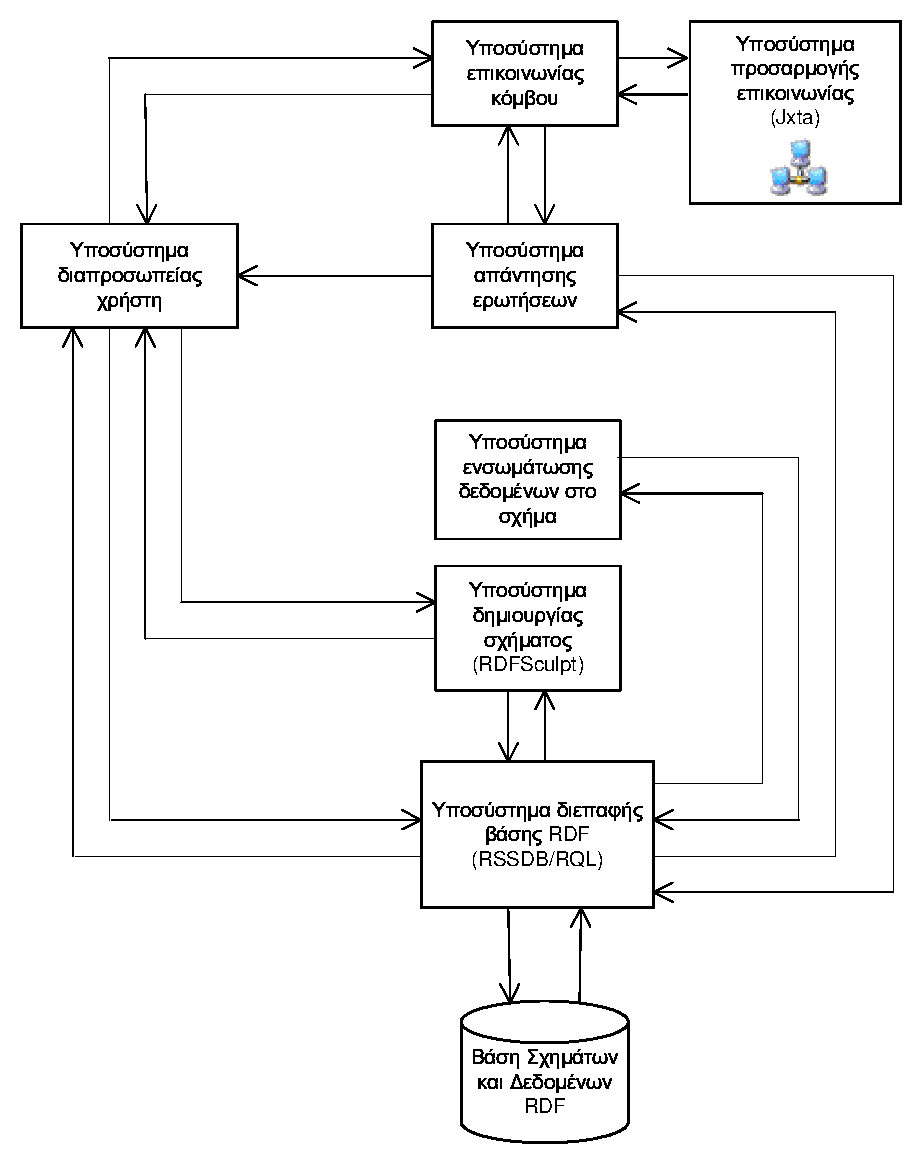
\includegraphics{figures/peerArchitecture.eps} 
    \caption{Αρχιτεκτονική Απλού Κόμβου}
    \label{figure4.1}
\end{figure} 

Το Σχήμα~\ref{figure4.1} απεικονίζει ..............


\subsection{Περιγραφή υποσυστημάτων}
Παρακάτω δίνεται λεπτομερής περιγραφή για καθένα από τα συστήματα
που αναφέραμε. Η περιγραφή αυτή γίνεται με βάση τα διαγράμματα
ροής δεδομένων.

\subsubsection{Υποσύστημα δημιουργίας σχήματος}
Το υποσύστημα αυτό ...............
	\chapter{Υλοποίηση}
\InitialCharacter{Σ}το κεφάλαιο αυτό περιγράφεται η υλοποίηση του συστήματος, με βάση τη μελέτη που παρουσιάστηκε στο προηγούμενο κεφάλαιο. Αρχικά παρουσιάζεται η πλατφόρμα και τα προγραμματιστικά εργαλεία που χρησιμοποιήθηκαν. Στη συνέχεια δίνονται οι λεπτομέρειες υλοποίησης για τους βασικούς αλγορίθμους του συστήματος καθώς και η δομή του κώδικα.

\section{Λεπτομέρειες υλοποίησης}
Στην ενότητα αυτή παρουσιάζονται οι βασικοί αλγόριθμοι που
αναπτύχθηκαν καθώς και λεπτομέρειες σχετικά με την υλοποίηση της
επικοινωνίας των κόμβων.

\subsection{Αλγόριθμοι}

\subsubsection{Αλγόριθμος εισαγωγής δεδομένων}
Όταν ένας κόμβος εισέρχεται για πρώτη φορά στο σύστημα, αρχικά
δημιουργεί το σχήμα που θέλει χρησιμοποιώντας το \en{RDFSculpt}.
Στη συνέχεια................

\noindent\textbf{Παράδειγμα} \\

Έστω ότι ο κόμβος έχει επιλέξει να συμμετέχει στο σύστημα με το \en{RDF} σχήμα που φαίνεται
στο Σχήμα. Έστω επίσης ότι από το \en{SQL} ερώτημα που έχει κάνει στη σχεσιακη
βάση, έχει προκύψει η όψη που φαίνεται στον Πίνακα. Για τις ανάγκες του παραδείγματος θεωρούμε
ότι η όψη αυτή περιέχει μόνο μία εγγραφή.

...........................

\section{Περιγραφή κλάσεων}
Στην ενότητα αυτή δίνεται μια σύντομη περιγραφή των κλάσεων,
των πεδίων και των μεθόδων που τις απαρτίζουν.

\subsection{\en{public class FirstUi}}
\noindent Η κλάση αυτή κατασκευάζει την οθόνη εισαγωγής του χρήστη στο σύστημα.\\

\noindent\textbf{Πεδία}

\begin{itemize}
\item\src{private GridBagLayout blayout} \\
Το \en{layout} για όλα τα \en{Panel}.
\item\src{private GridBagConstraints con} \\
Τα \en{constraints} για το \en{layout}.
\item\src{private Icon arrowR} \\
Εικονίδιο για το κουμπί \en{Next}.
\end{itemize}

\noindent\textbf{Μέθοδοι}

\begin{itemize}
\item\src{public FirstUi()}\\
Ο κατασκευαστής της κλάσης ο οποίος καλεί την \en{createEntryFrame()}.
\item\src{private void createEntryFrame()}\\
Μέθοδος που κατασκευάζει το en{frame}.
\end{itemize}
	\chapter{Έλεγχος}
\InitialCharacter{Σ}το κεφάλαιο αυτό γίνεται ο έλεγχος καλής λειτουργίας του συστήματος.

\section{Μεθοδολογία Ελέγχου}
Ο έλεγχος του συστήματος αυτού πραγματοποιήθηκε με τη χρήση ενός
σεναρίου λειτουργίας. Σύμφωνα με το σενάριο αυτό θεωρούμε ότι στο
σύστημα υπάρχουν τρεις κόμβοι (\en{peer1,peer2,peer3}). Θεωρούμε
επίσης ότι οι κόμβοι \en{peer2} και \en{peer3} έχουν ήδη σχήμα και
δεδομένα. Το σχήμα του \en{peer2} φαίνεται στο
Σχήμα.



Επίσης η τοπολογία του συστήματος έχει ως εξής: ο \en{peer2} είναι
γείτονας του \en{peer1} και ο \en{peer3} γείτονας του \en{peer2}.

Αρχικά λοιπόν θα δημιουργήσουμε σχήμα για τον κόμβο \en{peer1} και
στη συνέχεια θα εισάγουμε σε αυτό δεδομένα εξετάζοντας έτσι την
καλή λειτουργία του υποσυστήματος δημιουργίας σχήματος και του
υποσυστήματος εισαγωγής δεδομένων. Στη συνέχεια από τον κόμβο αυτό
στέλνουμε ερωτήσεις στους υπόλοιπους για τον έλεγχο του
υποσυστήματος απάντησης ερωτήσεων και επικοινωνίας κόμβων.

\section{Αναλυτική παρουσίαση ελέγχου}
Στην ενότητα αυτή παρουσιάζουμε αναλυτικά τον έλεγχο του
συστήματος σύμφωνα με το σενάριο που περιγράφηκε στην προηγούμενη
ενότητα.
	\chapter{Παράδειγμα Πίνακα}

\section{Συμπεράσματα}
Τα συστήματα ομότιμων κόμβων, προκειμένου να υποστηρίζουν πιο
εκφραστικές λειτουργίες αναπαράστασης και αναζήτησης δεδομένων,
εξελίχθηκαν στα συστήματα ομότιμων κόμβων τα οποία βασίζονται στις
τεχνολογίες του Σημασιολογικού Ιστού για την αναπαράσταση των
δεδομένων μέσω σχημάτων που τα περιγράφουν (\en{Schema-based
peer-to-peer systems}).

Συμπερασματικά το σύστημα που αναπτύχθηκε στα πλαίσια αυτής της
διπλωματικής είναι ένα πλήρες σύστημα ομότιμων κόμβων βασισμένο σε
σχήματα, το οποίο καθιστά δυνατή την αναζήτηση της πληροφορίας με
ένα διαφορετικό τρόπο απ' ότι τα προϋπάρχοντα  συστήματα.

\section{Μελλοντικές Επεκτάσεις}
Το σύστημα που αναπτύχθηκε στα πλαίσια αυτής της διπλωματικής
εργασίας θα μπορούσε να βελτιωθεί και να επεκταθεί περαιτέρω,
τουλάχιστον ως προς τρεις κατευθύνσεις. Συγκεκριμένα, αναφέρονται
τα ακόλουθα:

\begin{itemize}
\item Ενσωμάτωση διαδικασίας επιλογής σχήματος με βάση το οποίο ο
κόμβος θα συμμετέχει στο σύστημα. Έτσι όπως έχει σχεδιαστεί το
σύστημα, κάθε κόμβος έχει τη δυνατότητα να δημιουργήσει πολλά
σχήματα και να αποθηκεύσει δεδομένα σε περισσότερα από ένα. Ως
σχήμα του κόμβου (με βάση το οποίο απαντάει τις ερωτήσεις),
θεωρείται το τελευταίο στο οποίο αποθήκευσε δεδομένα. Η δυνατότητα
επιλογής θα του παρείχε περισσότερη ευελιξία.
\item Δυνατότητα αντιστοίχισης δεδομένων τα οποία να μην είναι
αποθηκευμένα σε βάση δεδομένων αλλά σε αρχεία. Η αποδέσμευση από
τη βάση δεδομένων θα έκανε το σύστημα πιο εύκολο στην εγκατάσταση
και τη χρήση.
\item Αξιολόγηση του συστήματος ως προς τη συμπεριφορά του αν
συμμετέχει σε αυτό μεγάλος αριθμός κόμβων \en{(scalability
testing)} και αν χρησιμοποιηθεί ένα πολύ μεγάλο καθολικό σχήμα. H
αξιολόγηση αυτή αφορά την ταχύτητα με την οποία ένας κόμβος
παίρνει απαντήσεις σε μια ερώτηση καθώς και την ποιότητα των
απαντήσεων.
\end{itemize}

%
	\begin{table}[!tb]
		\centering
		\caption{Πίνακας αλήθειας της λογικής συνάρτησης \en{F}}
		\small
		\renewcommand{\arraystretch}{1.3}
		\begin{tabular}{| c | c | c || c |}
			\hline               
		  	\textbf{\en{A}} & \textbf{\en{B}} &  \textbf{\en{C}} &   \textbf{\en{F}} \\
			\hline
				  0 & 0 & 0 & 0  \\
				  0 & 0 & 1 & 0  \\
				  0 & 1 & 0 & 1  \\
				  0 & 1 & 1 & 0  \\	
				  1 & 0 & 0 & 1  \\
				  1 & 0 & 1 & 0  \\
				  1 & 1 & 0 & 1  \\
				  1 & 1 & 1 & 0  \\
		  	\hline
		\end{tabular}
		\label{table07.01}
	\end{table}
%
	\chapter{Παράδειγμα Μαθηματικών Σχέσεων -- Εκφράσεων και Αλγορίθμων}

\section{Συμπεράσματα}
Τα συστήματα ομότιμων κόμβων, προκειμένου να υποστηρίζουν πιο
εκφραστικές λειτουργίες αναπαράστασης και αναζήτησης δεδομένων,
εξελίχθηκαν στα συστήματα ομότιμων κόμβων τα οποία βασίζονται στις
τεχνολογίες του Σημασιολογικού Ιστού για την αναπαράσταση των
δεδομένων μέσω σχημάτων που τα περιγράφουν (\en{Schema-based
peer-to-peer systems}).

Στα συστήματα αυτά κάθε \en{$\displaystyle y=\int_0^1f(x)dx$} \en{$y=\int_0^1f(x)dx$} κόμβος χρησιμοποιεί ένα σχήμα για την \en{$\displaystyle \sum_{i=0}^{100}a_i$}
αναπαράσταση των δεδομένων του. Όμως σε ένα σύστημα ομότιμων
κόμβων, κάθε κόμβος έχει διαφορετικές απαιτήσεις αναπαράστασης
δεδομένων. Επομένως πρέπει να υπάρχει ευελιξία στην επιλογή \en{$\displaystyle \frac{1}{1+x^2}$}
σχήματος. Τα συστήματα που έχουν προταθεί μέχρι τώρα και παρέχουν
αυτή την ευελιξία, για να είναι δυνατή η αναζήτηση πληροφορίας,
απαιτούν την ύπαρξη κανόνων αντιστοίχισης μεταξύ των σχημάτων με
βάση τους οποίους να μετασχηματίζονται οι ερωτήσεις. Όμως δεν
υποστηρίζεται ακόμα αυτόματη δημιουργία και δυναμική ανανέωση των
κανόνων, που είναι απαραίτητα για τα συστήματα ομότιμων κόμβων.
\begin{equation}
	y=\int_0^1f(x)dx
	\label{equation08.01}
\end{equation}

Η συνεισφορά της (\ref{equation08.01}) παρούσας διπλωματικής εργασίας έχει δύο σκέλη. Το
πρώτο αφορά τη δημιουργία ενός πλήρους συστήματος ομότιμων κόμβων
βασισμένο σε σχήματα \en{RDF} το οποίο παρέχει: (α) την υποδομή
για την επικοινωνία των κόμβων,(β) μηχανισμό δημιουργίας σχήματος,
(γ) μηχανισμό ενσωμάτωσης σχεσιακών δεδομένων στο σχήμα με τη
χρήση αντιστοιχίσεων που δημιουργεί ο χρήστης με τη βοήθεια
ειδικής διαπροσωπείας, (δ) ευέλικτη διαπροσωπεία χρήστη για τη
διατύπωση ερωτημάτων και (ε) μηχανισμό απάντησης και επεξεργασίας
ερωτήσεων.

Το δεύτερο σκέλος αφορά το γεγονός ότι το συγκεκριμένο σύστημα
προσφέρει μια σχετική ευελιξία ως προς την επιλογή του σχήματος
από τον κάθε κόμβο, ενώ ταυτόχρονα δίνει τη δυνατότητα
μετασχηματισμού ερωτήσεων χωρίς τη χρήση κανόνων αντιστοίχισης.
Συγκεκριμένα, τα σχήματα των κόμβων αποτελούν
υποσύνολα$-$όψεις$($\en{views}) ενός βασικού σχήματος που
ονομάζεται καθολικό σχήμα. Εκμεταλλευόμενοι λοιπόν το γεγονός ότι
τα σχήματα αυτά είναι συμβατά μεταξύ τους, έχουμε τη δυνατότητα
ελέγχου της ικανοποιησιμότητας μιας ερώτησης και μετατροπής της
όπου χρειάζεται, χρησιμοποιώντας τόσο το σχήμα του κόμβου όσο και
το καθολικό σχήμα.

Συμπερασματικά το σύστημα που αναπτύχθηκε στα πλαίσια αυτής της
διπλωματικής είναι ένα πλήρες σύστημα ομότιμων κόμβων βασισμένο σε
σχήματα, το οποίο καθιστά δυνατή την αναζήτηση της πληροφορίας με
ένα διαφορετικό τρόπο απ' ότι τα προϋπάρχοντα  συστήματα.

\section{Μελλοντικές Επεκτάσεις}
Το σύστημα που αναπτύχθηκε στα πλαίσια αυτής της διπλωματικής
εργασίας θα μπορούσε να βελτιωθεί και να επεκταθεί περαιτέρω,
τουλάχιστον ως προς τρεις κατευθύνσεις. Συγκεκριμένα, αναφέρονται
τα ακόλουθα:

%
\begin{algorithm}[tb]
  \caption{Μετατροπή δεκαδικού αριθμού σε δυαδικό, με τη μέθοδο των διαδοχικών διαιρέσεων με το 2}
  \label{decimal2binary1}
	\begin{algorithmic}
		\Require $X_{(10)}$ \small (\emph{ο δεκαδικός αριθμός προς μετατροπή}) \normalsize
		\Ensure $X_{(2)}$ \small (\emph{η δυαδική αναπαράσταση του Χ}) \normalsize
		\State Θέσε Δ=$X_{(10)}$ \small (\emph{Δ = διαιρετέος}) \normalsize
		\State Θέσε Π=1 \small (\emph{Π = πηλίκο}) \normalsize
		\State Θέσε $X_{(2)}$=<<>> \small (\emph{<<>> ο κενός χαρακτήρας}) \normalsize
		\While{Π$\neq$0}
			\State Διαίρεσε το Δ με το 2 και βρες το πηλίκο Π, και το υπόλοιπο υ.
			\State $X_{(2)}$=υ+$X_{(2)}$ \small (\emph{Τοποθέτησε το υπόλοιπο υ στα αριστερά του $X_{(2)}$}) \normalsize
			\State Θέσε Δ=Π \small (\emph{Το πηλίκο Π τίθεται ως διαιρετέος για την επόμενη διαίρεση}) \normalsize
		\EndWhile
	\end{algorithmic}
\end{algorithm}
%

%
\begin{algorithm}[tb]
  \caption{Κάποιος αλγόριθμος ...}
  \label{some_algorithm}
  \selectlanguage{english}
  \lstset{language=C}
  \begin{lstlisting}
#include <stdio.h>
#define N 10
/* Block
 * comment */
 
int main()
{
    int i;
 
    // Line comment.
    puts("Hello world!");
 
    for (i = 0; i < N; i++)
    {
        puts("LaTeX is also great for programmers!");
    }
 
    return 0;
}
  \end{lstlisting}
 \selectlanguage{greek}
\end{algorithm}
%

\begin{itemize}
\item Ενσωμάτωση διαδικασίας επιλογής σχήματος με βάση το οποίο ο
κόμβος θα συμμετέχει στο σύστημα. Έτσι όπως έχει σχεδιαστεί το
σύστημα, κάθε κόμβος έχει τη δυνατότητα να δημιουργήσει πολλά
σχήματα και να αποθηκεύσει δεδομένα σε περισσότερα από ένα. Ως
σχήμα του κόμβου (με βάση το οποίο απαντάει τις ερωτήσεις),
θεωρείται το τελευταίο στο οποίο αποθήκευσε δεδομένα. Η δυνατότητα
επιλογής θα του παρείχε περισσότερη ευελιξία.
\item Δυνατότητα αντιστοίχισης δεδομένων τα οποία να μην είναι
αποθηκευμένα σε βάση δεδομένων αλλά σε αρχεία. Η αποδέσμευση από
τη βάση δεδομένων θα έκανε το σύστημα πιο εύκολο στην εγκατάσταση
και τη χρήση.
\item Αξιολόγηση του συστήματος ως προς τη συμπεριφορά του αν
συμμετέχει σε αυτό μεγάλος αριθμός κόμβων \en{(scalability
testing)} και αν χρησιμοποιηθεί ένα πολύ μεγάλο καθολικό σχήμα. H
αξιολόγηση αυτή αφορά την ταχύτητα με την οποία ένας κόμβος
παίρνει απαντήσεις σε μια ερώτηση καθώς και την ποιότητα των
απαντήσεων.
\end{itemize}
    \part{Επίλογος}
	\chapter{Επίλογος}

\section{Συμπεράσματα}
Τα συστήματα ομότιμων κόμβων, προκειμένου να υποστηρίζουν πιο
εκφραστικές λειτουργίες αναπαράστασης και αναζήτησης δεδομένων,
εξελίχθηκαν στα συστήματα ομότιμων κόμβων τα οποία βασίζονται στις
τεχνολογίες του Σημασιολογικού Ιστού για την αναπαράσταση των
δεδομένων μέσω σχημάτων που τα περιγράφουν (\en{Schema-based
peer-to-peer systems}).

Στα συστήματα αυτά κάθε κόμβος χρησιμοποιεί ένα σχήμα για την
αναπαράσταση των δεδομένων του. Όμως σε ένα σύστημα ομότιμων
κόμβων, κάθε κόμβος έχει διαφορετικές απαιτήσεις αναπαράστασης
δεδομένων. Επομένως πρέπει να υπάρχει ευελιξία στην επιλογή
σχήματος. Τα συστήματα που έχουν προταθεί μέχρι τώρα και παρέχουν
αυτή την ευελιξία, για να είναι δυνατή η αναζήτηση πληροφορίας,
απαιτούν την ύπαρξη κανόνων αντιστοίχισης μεταξύ των σχημάτων με
βάση τους οποίους να μετασχηματίζονται οι ερωτήσεις. Όμως δεν
υποστηρίζεται ακόμα αυτόματη δημιουργία και δυναμική ανανέωση των
κανόνων, που είναι απαραίτητα για τα συστήματα ομότιμων κόμβων.

Η συνεισφορά της παρούσας διπλωματικής εργασίας έχει δύο σκέλη. Το
πρώτο αφορά τη δημιουργία ενός πλήρους συστήματος ομότιμων κόμβων
βασισμένο σε σχήματα \en{RDF} το οποίο παρέχει: (α) την υποδομή
για την επικοινωνία των κόμβων,(β) μηχανισμό δημιουργίας σχήματος,
(γ) μηχανισμό ενσωμάτωσης σχεσιακών δεδομένων στο σχήμα με τη
χρήση αντιστοιχίσεων που δημιουργεί ο χρήστης με τη βοήθεια
ειδικής διαπροσωπείας, (δ) ευέλικτη διαπροσωπεία χρήστη για τη
διατύπωση ερωτημάτων και (ε) μηχανισμό απάντησης και επεξεργασίας
ερωτήσεων.

Το δεύτερο σκέλος αφορά το γεγονός ότι το συγκεκριμένο σύστημα
προσφέρει μια σχετική ευελιξία ως προς την επιλογή του σχήματος
από τον κάθε κόμβο, ενώ ταυτόχρονα δίνει τη δυνατότητα
μετασχηματισμού ερωτήσεων χωρίς τη χρήση κανόνων αντιστοίχισης.
Συγκεκριμένα, τα σχήματα των κόμβων αποτελούν
υποσύνολα$-$όψεις$($\en{views}) ενός βασικού σχήματος που
ονομάζεται καθολικό σχήμα. Εκμεταλλευόμενοι λοιπόν το γεγονός ότι
τα σχήματα αυτά είναι συμβατά μεταξύ τους, έχουμε τη δυνατότητα
ελέγχου της ικανοποιησιμότητας μιας ερώτησης και μετατροπής της
όπου χρειάζεται, χρησιμοποιώντας τόσο το σχήμα του κόμβου όσο και
το καθολικό σχήμα.

Συμπερασματικά το σύστημα που αναπτύχθηκε στα πλαίσια αυτής της
διπλωματικής είναι ένα πλήρες σύστημα ομότιμων κόμβων βασισμένο σε
σχήματα, το οποίο καθιστά δυνατή την αναζήτηση της πληροφορίας με
ένα διαφορετικό τρόπο απ' ότι τα προϋπάρχοντα  συστήματα.

\section{Μελλοντικές Επεκτάσεις}
Το σύστημα που αναπτύχθηκε στα πλαίσια αυτής της διπλωματικής
εργασίας θα μπορούσε να βελτιωθεί και να επεκταθεί περαιτέρω,
τουλάχιστον ως προς τρεις κατευθύνσεις. Συγκεκριμένα, αναφέρονται
τα ακόλουθα:

\begin{itemize}
\item Ενσωμάτωση διαδικασίας επιλογής σχήματος με βάση το οποίο ο
κόμβος θα συμμετέχει στο σύστημα. Έτσι όπως έχει σχεδιαστεί το
σύστημα, κάθε κόμβος έχει τη δυνατότητα να δημιουργήσει πολλά
σχήματα και να αποθηκεύσει δεδομένα σε περισσότερα από ένα. Ως
σχήμα του κόμβου (με βάση το οποίο απαντάει τις ερωτήσεις),
θεωρείται το τελευταίο στο οποίο αποθήκευσε δεδομένα. Η δυνατότητα
επιλογής θα του παρείχε περισσότερη ευελιξία.
\item Δυνατότητα αντιστοίχισης δεδομένων τα οποία να μην είναι
αποθηκευμένα σε βάση δεδομένων αλλά σε αρχεία. Η αποδέσμευση από
τη βάση δεδομένων θα έκανε το σύστημα πιο εύκολο στην εγκατάσταση
και τη χρήση.
\item Αξιολόγηση του συστήματος ως προς τη συμπεριφορά του αν
συμμετέχει σε αυτό μεγάλος αριθμός κόμβων \en{(scalability
testing)} και αν χρησιμοποιηθεί ένα πολύ μεγάλο καθολικό σχήμα. H
αξιολόγηση αυτή αφορά την ταχύτητα με την οποία ένας κόμβος
παίρνει απαντήσεις σε μια ερώτηση καθώς και την ποιότητα των
απαντήσεων.
\end{itemize}
% Παραρτήματα
	\appendices
	\chapter{Παράδειγμα  Παραρτήματος}

\section{Πρώτη ενότητα}
Τα συστήματα ομότιμων κόμβων, προκειμένου να υποστηρίζουν πιο
εκφραστικές λειτουργίες αναπαράστασης και αναζήτησης δεδομένων,
εξελίχθηκαν στα συστήματα ομότιμων κόμβων τα οποία βασίζονται στις
τεχνολογίες του Σημασιολογικού Ιστού για την αναπαράσταση των
δεδομένων μέσω σχημάτων που τα περιγράφουν (\en{Schema-based
peer-to-peer systems}).

Συμπερασματικά το σύστημα που αναπτύχθηκε στα πλαίσια αυτής της
διπλωματικής είναι ένα πλήρες σύστημα ομότιμων κόμβων βασισμένο σε
σχήματα, το οποίο καθιστά δυνατή την αναζήτηση της πληροφορίας με
ένα διαφορετικό τρόπο απ' ότι τα προϋπάρχοντα  συστήματα.

\section{Μελλοντικές Επεκτάσεις}
Το σύστημα που αναπτύχθηκε στα πλαίσια αυτής της διπλωματικής
εργασίας θα μπορούσε να βελτιωθεί και να επεκταθεί περαιτέρω,
τουλάχιστον ως προς τρεις κατευθύνσεις. Συγκεκριμένα, αναφέρονται
τα ακόλουθα:

\begin{itemize}
\item Ενσωμάτωση διαδικασίας επιλογής σχήματος με βάση το οποίο ο
κόμβος θα συμμετέχει στο σύστημα. Έτσι όπως έχει σχεδιαστεί το
σύστημα, κάθε κόμβος έχει τη δυνατότητα να δημιουργήσει πολλά
σχήματα και να αποθηκεύσει δεδομένα σε περισσότερα από ένα. Ως
σχήμα του κόμβου (με βάση το οποίο απαντάει τις ερωτήσεις),
θεωρείται το τελευταίο στο οποίο αποθήκευσε δεδομένα. Η δυνατότητα
επιλογής θα του παρείχε περισσότερη ευελιξία.
\item Δυνατότητα αντιστοίχισης δεδομένων τα οποία να μην είναι
αποθηκευμένα σε βάση δεδομένων αλλά σε αρχεία. Η αποδέσμευση από
τη βάση δεδομένων θα έκανε το σύστημα πιο εύκολο στην εγκατάσταση
και τη χρήση.
\item Αξιολόγηση του συστήματος ως προς τη συμπεριφορά του αν
συμμετέχει σε αυτό μεγάλος αριθμός κόμβων \en{(scalability
testing)} και αν χρησιμοποιηθεί ένα πολύ μεγάλο καθολικό σχήμα. H
αξιολόγηση αυτή αφορά την ταχύτητα με την οποία ένας κόμβος
παίρνει απαντήσεις σε μια ερώτηση καθώς και την ποιότητα των
απαντήσεων.
\end{itemize}

%
	\begin{table}[!tb]
		\centering
		\caption{Πίνακας αλήθειας της λογικής συνάρτησης \en{F}}
		\small
		\renewcommand{\arraystretch}{1.3}
		\begin{tabular}{| c | c | c || c |}
			\hline               
		  	\textbf{\en{A}} & \textbf{\en{B}} &  \textbf{\en{C}} &   \textbf{\en{F}} \\
			\hline
				  0 & 0 & 0 & 0  \\
				  0 & 0 & 1 & 0  \\
				  0 & 1 & 0 & 1  \\
				  0 & 1 & 1 & 0  \\	
				  1 & 0 & 0 & 1  \\
				  1 & 0 & 1 & 0  \\
				  1 & 1 & 0 & 1  \\
				  1 & 1 & 1 & 0  \\
		  	\hline
		\end{tabular}
		\label{table_appA.01}
	\end{table}
%
	\chapter{Απόδειξη της σχέσης (8.1)}
Στο κεφάλαιο αυτό παρουσιάζεται η μελέτη που έγινε για την
υλοποίηση του συστήματος. Αρχικά περιγράφεται η αρχιτεκτονική του
συστήματος και γίνεται ο διαχωρισμός του στα επιμέρους
υποσυστήματα, ενώ στη συνέχεια περιγράφονται οι εφαρμογές του
συστήματος. \expandafter\textgreek{ελένη}

\section{Ανάλυση - περιγραφή αρχιτεκτονικής}
Στην ενότητα αυτή παρουσιάζεται η ανάλυση του συστήματος και ο
χωρισμός του σε υποσυστήματα όσον αφορά την αρχιτεκτονική.

\subsection{Διαχωρισμός υποσυστημάτων}
Το σύστημα αποτελείται από τους απλούς κόμβους και ένα κόμβο
διαχειριστή. Στο σημείο αυτό αναλύουμε το σύστημα ενός απλού
κόμβου, το οποίο αποτελείται από τα εξής υποσυστήματα:

\begin{itemize}
\item Υποσύστημα δημιουργίας σχήματος.
\item Υποσύστημα ενσωμάτωσης δεδομένων στο σχήμα.
\item Υποσύστημα επικοινωνίας κόμβου.
\end{itemize}


\begin{figure}[!ht] \centering
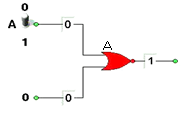
\includegraphics{figures/2.png} \caption{Προσομοίωση Πύλης \en{NOR}}\label{figureB.1}
\end{figure}

Το Σχήμα~\ref{figureB.1} απεικονίζει .................


\subsection{Περιγραφή υποσυστημάτων}
Παρακάτω δίνεται λεπτομερής περιγραφή για καθένα από τα συστήματα
που αναφέραμε. Η περιγραφή αυτή γίνεται με βάση τα διαγράμματα
ροής δεδομένων.

\subsubsection{Υποσύστημα δημιουργίας σχήματος}
Το υποσύστημα αυτό ...............
    \chapter{Παραδείγματα Βιβλιογραφικών Αναφορών}

\begin{center}
	\begin{tabular}{|c|c|}
    	\hline
    	\textbf{Τύπος βιβλιογραφικής πηγής} & \textbf{Αριθμός αναφοράς} \\
    	\hline\hline
    	Βιβλίο ξενόγλωσσο &  \cite{goossens93} \\
    	\hline
    	Βιβλίο ελληνικό &  \cite{greekbook} \\
    	\hline
    	Άρθρο σε επιστημονικό περιοδικό &  \cite{LiArTs13} \\
    	\hline
    	Παρουσίαση σε επιστημονικό συνέδριο &  \cite{dcis2011} \\
    	\hline
    	Ιστοσελίδα &  \cite{LaTeXProject} \\
    	\hline
    	Διπλωματική εργασία &  \cite{zoi04} \\
    	\hline
    	Πτυχιακή εργασία &  \cite{elli05} \\
    	\hline
    	Μεταπτυχιακή διπλωματική εργασία &  \cite{master04} \\
    	\hline
    	Διδακτορική διατριβή &  \cite{phd045} \\
    	\hline
    	Δίπλωμα ευρεσιτεχνίας (πατέντα) &  \cite{viswanathan2014convenient} \\
    	\hline
    	Τεχνική αναφορά &  \cite{MSU-CSE-05-29} \\
    	\hline
    \end{tabular}
\end{center}

          


    \chapter{Δημιουργία Ευρετηρίου}
Δείτε το περιεχόμενο του αρχείου \en{appD.tex} για τρόπους ορισμού ελληνικών και ξενόγλωσσων όρων ευρετηρίου.

% Παραδείγματα ξενόγλωσσων όρων
\indexEN{xerox} \indexEN{babel} \indexEN{anna} \indexEN{babylon}

% Παραδείγματα ελληνικών όρων (προσέξτε τη χρήση λατινικού προθέματος για τη σωστή ταξινόμηση των όρων) 
\indexGR{P@πτυχιακή} \indexGR{E@έλενα} \indexGR{E@ελένη} \indexGR{X@χρώμα} \indexGR{R@ροή} \indexGR{Z@ώριμος} \indexGR{A@άννα} 

    \chapter{Εισαγωγή Εικόνων}
Δείτε το περιεχόμενο του αρχείου \en{appE.tex} για τον τρόπο εισαγωγής εικόνων.

\begin{Illustration}[!h] 
	\centering
	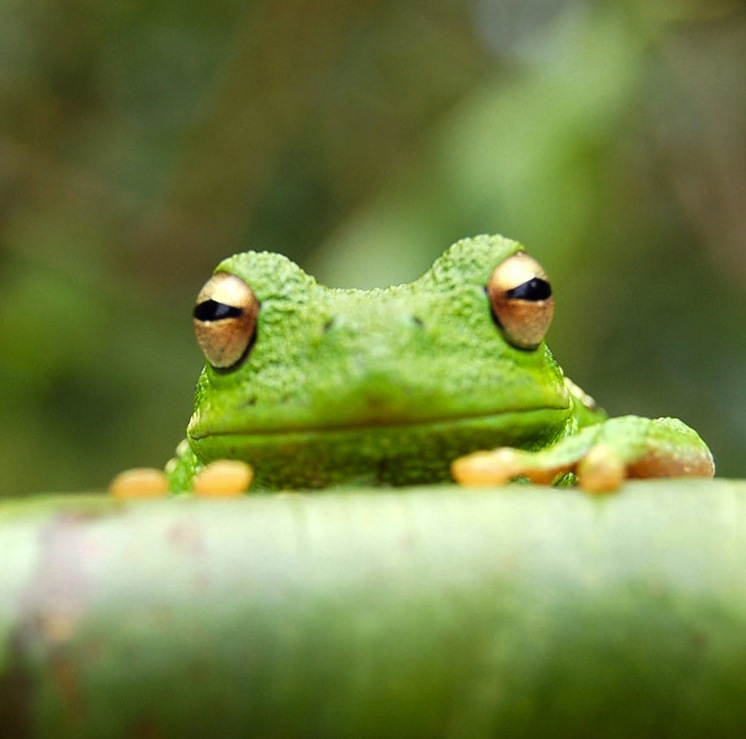
\includegraphics[width=0.5\textwidth]{figures/frog.jpg} 
	\caption{Βάτραχος}
	\label{frog_image}
\end{Illustration}
 
% Βιβλιογραφία - Αναφορές
	\bibliography{references}
% Συντομογραφίες - Αρκτικόλεξα - Ακρωνύμια
	\includeabbreviations{back_matter/abbreviations}
% Γλωσσάριο
	\includeglossary{back_matter/glossary}
%%%%%%%%%%%%%%%%%%%%%%%%%%%%%%%%%%%%%%%%%%%%%%%%%%%%
% Ευρετήριο Όρων
	\printindices
%
%%%%%%%%%%%%%%%%%%
%%%%%%%%%%%%%%%%%%

%% Δημιουργία ετικετών CD:

	\definecdlabeloffsets{0}{-0.65}{0}{0.55} % upper label x offset [cm] (default=0) /  upper label y offset [cm] (default=0) /  lower label x offset [cm] (default=0) /  lower  label y offset [cm] (default=0) -- For Q-Connect KF01579 labels use the following offset values: {0}{-0.65}{0}{0.55}

	\createcdlabel{Πρότυπο Σύστημα Ομότιμων \\ Κόμβων Βασισμένο σε Σχήματα \en{RDF}}{Κωνσταντίνος Δ. Δημητρίου}{ΟΚΤΩΒΡΙΟΣ}{2020}{8} % τίτλος διπλωματικής / όνομα συγγραφέα / μήνας / έτος / εύρος περιοχής τίτλου σε cm (προτεινόμενη τιμή: 8) 

%%σ
%% Δημιουργία εξωφύλλου θήκης CD:

	\createcdcover{Πρότυπο Σύστημα Ομότιμων \\ Κόμβων Βασισμένο σε Σχήματα \en{RDF}}{Στάμος Φ. Ευάγγελος}{ΟΚΤΩΒΡΙΟΣ}{2020}{10} % τίτλος πτυχιακής / όνομα συγγραφέα / μήνας / έτος / εύρος περιοχής τίτλου σε cm (προτεινόμενη τιμή: 10) 

%%
%
\end{document}

%%%%%%%%%%%%%%%%%%%%%%%%%%%%%%%%%%%%%%%%%%%%%%%%%%%%
